\documentclass[twoside]{book}

% Packages required by doxygen
\usepackage{fixltx2e}
\usepackage{calc}
\usepackage{doxygen}
\usepackage[export]{adjustbox} % also loads graphicx
\usepackage{graphicx}
\usepackage[utf8]{inputenc}
\usepackage{makeidx}
\usepackage{multicol}
\usepackage{multirow}
\PassOptionsToPackage{warn}{textcomp}
\usepackage{textcomp}
\usepackage[nointegrals]{wasysym}
\usepackage[table]{xcolor}

% Font selection
\usepackage[T1]{fontenc}
\usepackage[scaled=.90]{helvet}
\usepackage{courier}
\usepackage{amssymb}
\usepackage{sectsty}
\renewcommand{\familydefault}{\sfdefault}
\allsectionsfont{%
  \fontseries{bc}\selectfont%
  \color{darkgray}%
}
\renewcommand{\DoxyLabelFont}{%
  \fontseries{bc}\selectfont%
  \color{darkgray}%
}
\newcommand{\+}{\discretionary{\mbox{\scriptsize$\hookleftarrow$}}{}{}}

% Page & text layout
\usepackage{geometry}
\geometry{%
  a4paper,%
  top=2.5cm,%
  bottom=2.5cm,%
  left=2.5cm,%
  right=2.5cm%
}
\tolerance=750
\hfuzz=15pt
\hbadness=750
\setlength{\emergencystretch}{15pt}
\setlength{\parindent}{0cm}
\setlength{\parskip}{0.2cm}
\makeatletter
\renewcommand{\paragraph}{%
  \@startsection{paragraph}{4}{0ex}{-1.0ex}{1.0ex}{%
    \normalfont\normalsize\bfseries\SS@parafont%
  }%
}
\renewcommand{\subparagraph}{%
  \@startsection{subparagraph}{5}{0ex}{-1.0ex}{1.0ex}{%
    \normalfont\normalsize\bfseries\SS@subparafont%
  }%
}
\makeatother

% Headers & footers
\usepackage{fancyhdr}
\pagestyle{fancyplain}
\fancyhead[LE]{\fancyplain{}{\bfseries\thepage}}
\fancyhead[CE]{\fancyplain{}{}}
\fancyhead[RE]{\fancyplain{}{\bfseries\leftmark}}
\fancyhead[LO]{\fancyplain{}{\bfseries\rightmark}}
\fancyhead[CO]{\fancyplain{}{}}
\fancyhead[RO]{\fancyplain{}{\bfseries\thepage}}
\fancyfoot[LE]{\fancyplain{}{}}
\fancyfoot[CE]{\fancyplain{}{}}
\fancyfoot[RE]{\fancyplain{}{\bfseries\scriptsize Generated on Fri Apr 24 2015 12\+:05\+:55 for My Project by Doxygen }}
\fancyfoot[LO]{\fancyplain{}{\bfseries\scriptsize Generated on Fri Apr 24 2015 12\+:05\+:55 for My Project by Doxygen }}
\fancyfoot[CO]{\fancyplain{}{}}
\fancyfoot[RO]{\fancyplain{}{}}
\renewcommand{\footrulewidth}{0.4pt}
\renewcommand{\chaptermark}[1]{%
  \markboth{#1}{}%
}
\renewcommand{\sectionmark}[1]{%
  \markright{\thesection\ #1}%
}

% Indices & bibliography
\usepackage{natbib}
\usepackage[titles]{tocloft}
\setcounter{tocdepth}{3}
\setcounter{secnumdepth}{5}
\makeindex

% Hyperlinks (required, but should be loaded last)
\usepackage{ifpdf}
\ifpdf
  \usepackage[pdftex,pagebackref=true]{hyperref}
\else
  \usepackage[ps2pdf,pagebackref=true]{hyperref}
\fi
\hypersetup{%
  colorlinks=true,%
  linkcolor=blue,%
  citecolor=blue,%
  unicode%
}

% Custom commands
\newcommand{\clearemptydoublepage}{%
  \newpage{\pagestyle{empty}\cleardoublepage}%
}


%===== C O N T E N T S =====

\begin{document}

% Titlepage & ToC
\hypersetup{pageanchor=false,
             bookmarks=true,
             bookmarksnumbered=true,
             pdfencoding=unicode
            }
\pagenumbering{roman}
\begin{titlepage}
\vspace*{7cm}
\begin{center}%
{\Large My Project }\\
\vspace*{1cm}
{\large Generated by Doxygen 1.8.9.1}\\
\vspace*{0.5cm}
{\small Fri Apr 24 2015 12:05:55}\\
\end{center}
\end{titlepage}
\clearemptydoublepage
\tableofcontents
\clearemptydoublepage
\pagenumbering{arabic}
\hypersetup{pageanchor=true}

%--- Begin generated contents ---
\chapter{kvalifikatsioon-\/dodger}
\label{md__c_1__users_kasutaja__desktop__simo__proge_python_kvalifikatsioon-dodger__r_e_a_d_m_e}
\hypertarget{md__c_1__users_kasutaja__desktop__simo__proge_python_kvalifikatsioon-dodger__r_e_a_d_m_e}{}
väike mäng kvalifikatsiooni jaoks 
\chapter{Hierarchical Index}
\section{Class Hierarchy}
This inheritance list is sorted roughly, but not completely, alphabetically\+:\begin{DoxyCompactList}
\item Sprite\begin{DoxyCompactList}
\item \contentsline{section}{classes.\+obstacle}{\pageref{classclasses_1_1obstacle}}{}
\item \contentsline{section}{classes.\+Ship}{\pageref{classclasses_1_1_ship}}{}
\end{DoxyCompactList}
\end{DoxyCompactList}

\chapter{Class Index}
\section{Class List}
Here are the classes, structs, unions and interfaces with brief descriptions\+:\begin{DoxyCompactList}
\item\contentsline{section}{\hyperlink{classclasses_1_1obstacle}{classes.\+obstacle} }{\pageref{classclasses_1_1obstacle}}{}
\item\contentsline{section}{\hyperlink{classclasses_1_1_ship}{classes.\+Ship} }{\pageref{classclasses_1_1_ship}}{}
\end{DoxyCompactList}

\chapter{Class Documentation}
\hypertarget{classclasses_1_1obstacle}{}\section{classes.\+obstacle Class Reference}
\label{classclasses_1_1obstacle}\index{classes.\+obstacle@{classes.\+obstacle}}
Inheritance diagram for classes.\+obstacle\+:\begin{figure}[H]
\begin{center}
\leavevmode
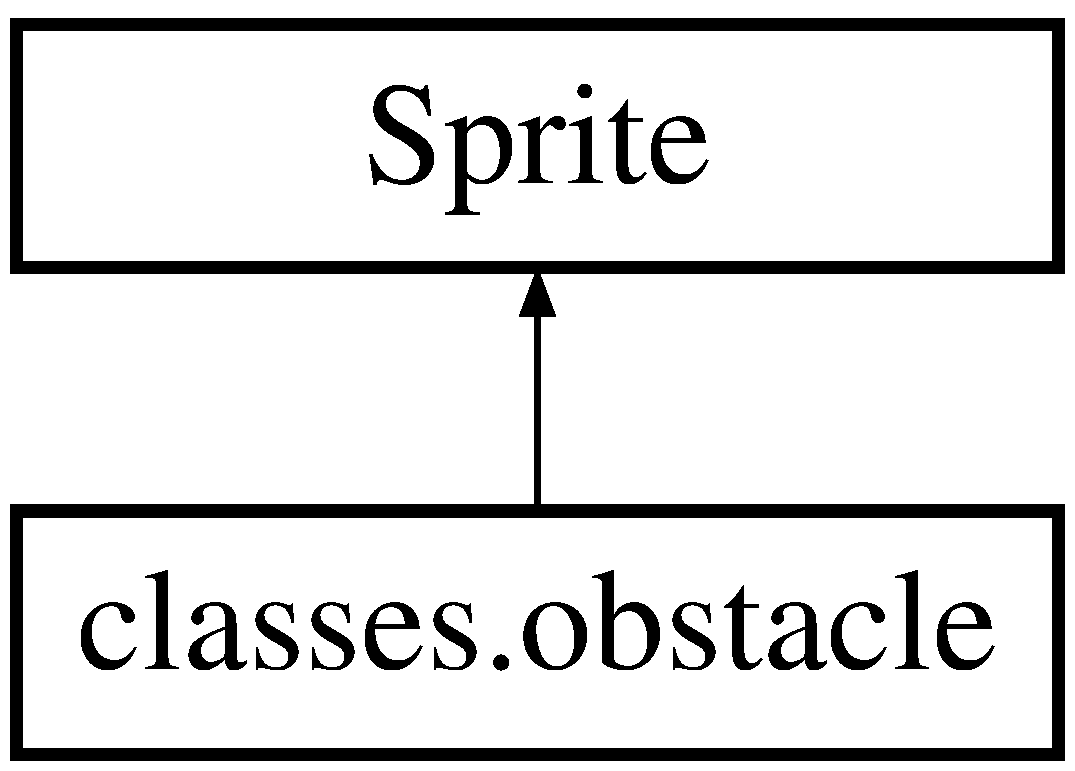
\includegraphics[height=2.000000cm]{classclasses_1_1obstacle}
\end{center}
\end{figure}
\subsection*{Public Member Functions}
\begin{DoxyCompactItemize}
\item 
\hypertarget{classclasses_1_1obstacle_a1267f3775feb3a38993eaf7c06b70e0b}{}def {\bfseries \+\_\+\+\_\+init\+\_\+\+\_\+} (self)\label{classclasses_1_1obstacle_a1267f3775feb3a38993eaf7c06b70e0b}

\item 
\hypertarget{classclasses_1_1obstacle_a21704232a6fd57b771888202200302e7}{}def {\bfseries rand\+\_\+data\+\_\+calc} (self)\label{classclasses_1_1obstacle_a21704232a6fd57b771888202200302e7}

\item 
\hypertarget{classclasses_1_1obstacle_a7359254ed2a6b4f4860420c34a8dde11}{}def {\bfseries update} (self)\label{classclasses_1_1obstacle_a7359254ed2a6b4f4860420c34a8dde11}

\end{DoxyCompactItemize}
\subsection*{Public Attributes}
\begin{DoxyCompactItemize}
\item 
\hypertarget{classclasses_1_1obstacle_afb097093e25efbe66b816fbfe8e595a3}{}{\bfseries screen}\label{classclasses_1_1obstacle_afb097093e25efbe66b816fbfe8e595a3}

\item 
\hypertarget{classclasses_1_1obstacle_ad57e5c1104ac75b5117d5a4cbb4c8707}{}{\bfseries image}\label{classclasses_1_1obstacle_ad57e5c1104ac75b5117d5a4cbb4c8707}

\item 
\hypertarget{classclasses_1_1obstacle_a2ed6dce87e174487e5c3e10ef7dff7aa}{}{\bfseries rand\+\_\+scale}\label{classclasses_1_1obstacle_a2ed6dce87e174487e5c3e10ef7dff7aa}

\item 
\hypertarget{classclasses_1_1obstacle_a53ca65f2c8f91c55679dce75bf6fec3b}{}{\bfseries rand\+\_\+speed}\label{classclasses_1_1obstacle_a53ca65f2c8f91c55679dce75bf6fec3b}

\item 
\hypertarget{classclasses_1_1obstacle_a5f8bdd4f404148f9a19e416fb8d2c1d6}{}{\bfseries rand\+\_\+loc}\label{classclasses_1_1obstacle_a5f8bdd4f404148f9a19e416fb8d2c1d6}

\item 
\hypertarget{classclasses_1_1obstacle_ab67a18a8d5e47419be009b51ba42b9aa}{}{\bfseries rect}\label{classclasses_1_1obstacle_ab67a18a8d5e47419be009b51ba42b9aa}

\end{DoxyCompactItemize}


\subsection{Detailed Description}
\begin{DoxyVerb}Obstacles on the way of the ship
Returns: obstacle object
Functions: init, update, rand_data_calc, stop
Attributes: speed, image, location, scale\end{DoxyVerb}
 

The documentation for this class was generated from the following file\+:\begin{DoxyCompactItemize}
\item 
C\+:/\+Users/kasutaja/\+Desktop/\+Simo/\+Proge/python/kvalifikatsioon-\/dodger/classes.\+py\end{DoxyCompactItemize}

\hypertarget{classclasses_1_1_ship}{}\section{classes.\+Ship Class Reference}
\label{classclasses_1_1_ship}\index{classes.\+Ship@{classes.\+Ship}}
Inheritance diagram for classes.\+Ship\+:\begin{figure}[H]
\begin{center}
\leavevmode
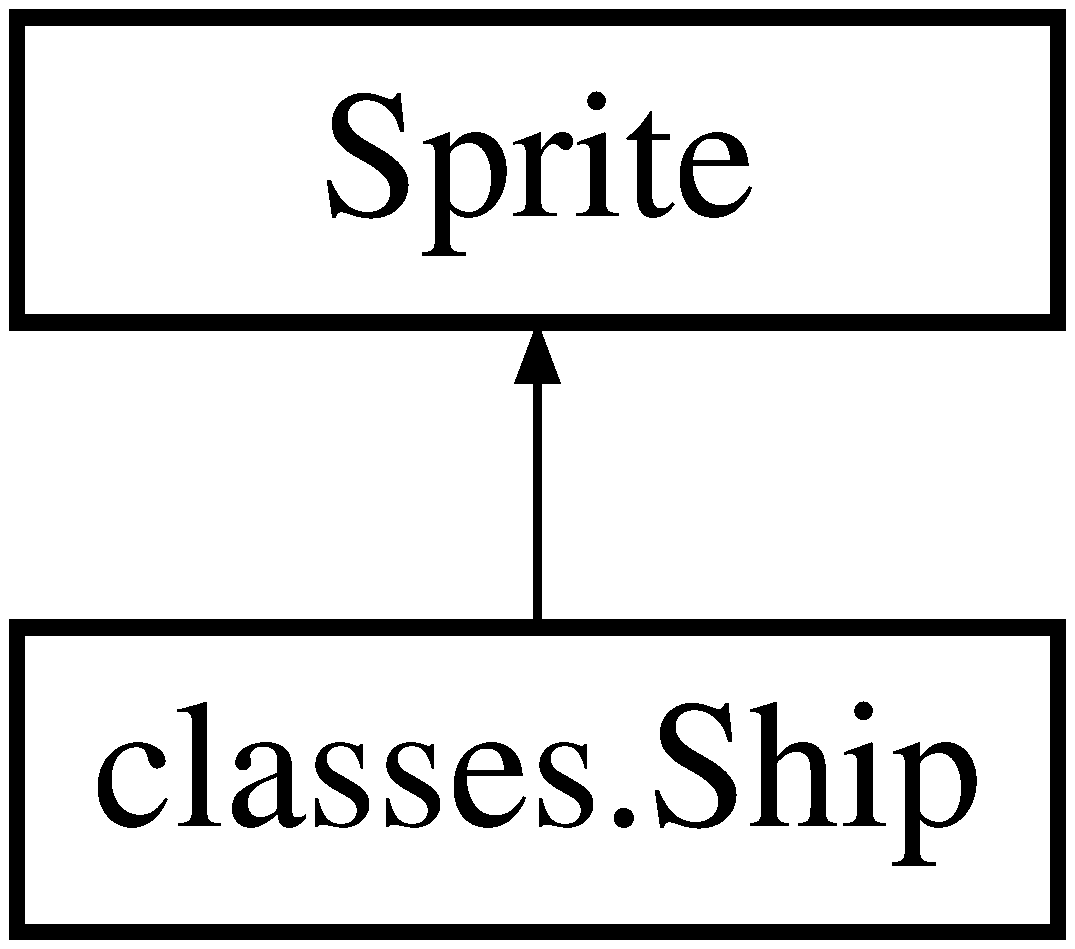
\includegraphics[height=2.000000cm]{classclasses_1_1_ship}
\end{center}
\end{figure}
\subsection*{Public Member Functions}
\begin{DoxyCompactItemize}
\item 
\hypertarget{classclasses_1_1_ship_adf2eb54de7bb8df098cf6c4134a6d186}{}def {\bfseries \+\_\+\+\_\+init\+\_\+\+\_\+} (self, speed)\label{classclasses_1_1_ship_adf2eb54de7bb8df098cf6c4134a6d186}

\item 
\hypertarget{classclasses_1_1_ship_ac1a587b0beba11d416d58758335ae223}{}def {\bfseries reinit} (self)\label{classclasses_1_1_ship_ac1a587b0beba11d416d58758335ae223}

\item 
\hypertarget{classclasses_1_1_ship_a82f0d397e08683e8fc166381ccf37844}{}def {\bfseries update} (self)\label{classclasses_1_1_ship_a82f0d397e08683e8fc166381ccf37844}

\item 
\hypertarget{classclasses_1_1_ship_a70a990236bce1668a4934ddedd6bec53}{}def {\bfseries moveleft} (self)\label{classclasses_1_1_ship_a70a990236bce1668a4934ddedd6bec53}

\item 
\hypertarget{classclasses_1_1_ship_a5986dca8d7637d2aafd4db4251e7b837}{}def {\bfseries moveright} (self)\label{classclasses_1_1_ship_a5986dca8d7637d2aafd4db4251e7b837}

\item 
\hypertarget{classclasses_1_1_ship_a8ccdbfec96ec67ff27ef2afa6e30bab3}{}def {\bfseries stop} (self)\label{classclasses_1_1_ship_a8ccdbfec96ec67ff27ef2afa6e30bab3}

\end{DoxyCompactItemize}
\subsection*{Public Attributes}
\begin{DoxyCompactItemize}
\item 
\hypertarget{classclasses_1_1_ship_aaa521a3e5eb9c1226fbe86fe0665561a}{}{\bfseries image}\label{classclasses_1_1_ship_aaa521a3e5eb9c1226fbe86fe0665561a}

\item 
\hypertarget{classclasses_1_1_ship_ab95eccff4a54cc2e6589a8231f81dbc9}{}{\bfseries rect}\label{classclasses_1_1_ship_ab95eccff4a54cc2e6589a8231f81dbc9}

\item 
\hypertarget{classclasses_1_1_ship_ab76b7616c30c5e11956259958fc7f8f0}{}{\bfseries orig\+\_\+rect\+\_\+x}\label{classclasses_1_1_ship_ab76b7616c30c5e11956259958fc7f8f0}

\item 
\hypertarget{classclasses_1_1_ship_a645f11e76bb14435a6c64128e0719dba}{}{\bfseries orig\+\_\+rect\+\_\+y}\label{classclasses_1_1_ship_a645f11e76bb14435a6c64128e0719dba}

\item 
\hypertarget{classclasses_1_1_ship_a05c797390e75307b7c1c149de9d76ce7}{}{\bfseries speed\+\_\+num}\label{classclasses_1_1_ship_a05c797390e75307b7c1c149de9d76ce7}

\item 
\hypertarget{classclasses_1_1_ship_ab652b59eb8c66b74f5f0d36e22637414}{}{\bfseries speed}\label{classclasses_1_1_ship_ab652b59eb8c66b74f5f0d36e22637414}

\end{DoxyCompactItemize}


\subsection{Detailed Description}
\begin{DoxyVerb}Movable ship with which played dodges obstacles
Returns: ship object
Functions: init, reinit, update, moveleft, moveright, stop
Attributes: speed, location, image\end{DoxyVerb}
 

The documentation for this class was generated from the following file\+:\begin{DoxyCompactItemize}
\item 
C\+:/\+Users/kasutaja/\+Desktop/\+Simo/\+Proge/python/kvalifikatsioon-\/dodger/classes.\+py\end{DoxyCompactItemize}

%--- End generated contents ---

% Index
\backmatter
\newpage
\phantomsection
\clearemptydoublepage
\addcontentsline{toc}{chapter}{Index}
\printindex

\end{document}
